In this chapter experiments with real servos will be conducted in order to, firstly, tune the parameters of the simulation (servo's characteristics) and, secondly, verify that the simulation correctly predicts the behaviour of a real-life configuration.

\section{Problem statement}
Before using our simulator to test control algorithms it is useful to first verify that it gives physically accurate results. It would be a waste of time to conduct tests on a model that does not behave in the same way as the original does.

\section{Experimental set-up}
The set-up is explained in \cref{fig:exp_setup}. In later experiments a camera will be used to film the motion of the servos and compare it to the results of the simulation that is supposed to predict it.

\begin{figure}[htp]
\center
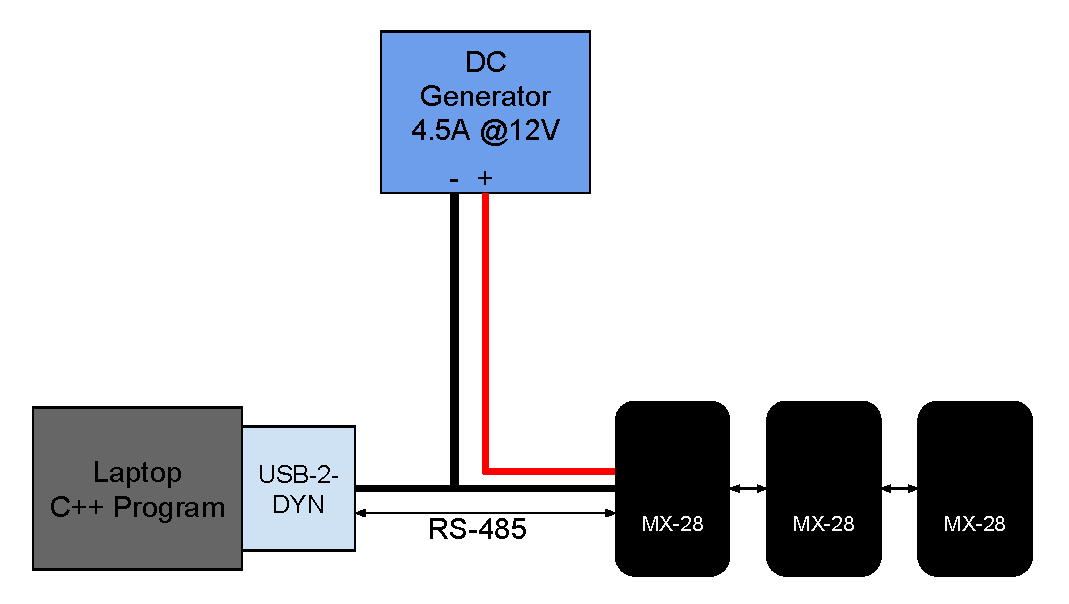
\includegraphics[width=0.6\textwidth]{figures/exp_setup}
\caption[Experimental setup]{Experimental setup : The MX-28 servos are powered by a DC generator and controlled by a laptop equipped with a USB2DYNAMIXEL(USB-2-DYN) device.}
\label{fig:exp_setup}
\end{figure}

\begin{figure}[htp]
\center
    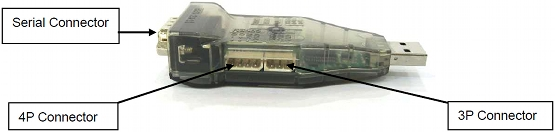
\includegraphics[width = 0.8\textwidth]{figures/u2d}
    \caption[USB2DYNAMIXEL]{Picture of a USB2DYNAMIXEL device. It turns an USB port into a serial port (RS485, TTL or classic serial connector) that can be used to control Dynamixel manufactured servos. [Taken from \url{http://support.robotis.com/en/product/auxdevice/interface/usb2dxl_manual.htm}]}
    \label{fig:usb2dyn}
\end{figure}

\section{Experiment 1 \label{sec:exp1}}
The purpose of the first experiment is to test the torque : to that end, a frame is fixed onto a single servo and weighted. The setup is represented on \cref{fig:exp1}.

\begin{figure}[htp]
\center
    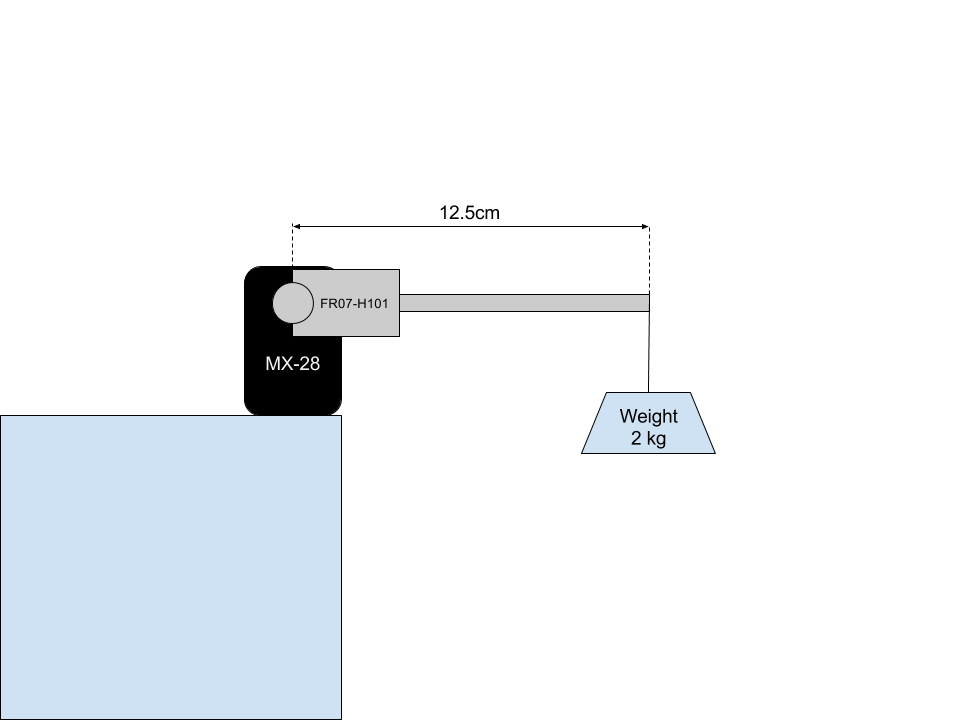
\includegraphics[width = 0.5\textwidth]{figures/exp1}
    \caption[Experimental setup for torque testing]{Experimental setup for torque testing. A weight $w$ of is suspended at a distance $d$ from the servo, resulting in a applied torque of $w \times g \times d$. The goal consists in finding the weight $w$ for which the servo is unable to lift the arm.}
    \label{fig:exp1}
\end{figure}

In our case, $d$ was equal to $22.5cm$ and we could reach a weight $w$ of $740g$ at $14.8V$. This equals to a torque of $1.64Ncm$. The complete results are listed in \cref{table:exp1_results}.
\begin{table}[htp]
\center
\begin{tabularx}{\textwidth}{@{}l X X X @{}}
\toprule
& \textbf{Stall torque @11.1V $[N.m]$} & \textbf{Stall torque @12V $[N.m]$} & \textbf{Stall torque @14.8V $[N.m]$}\\ 
\midrule
\textbf{Theoretical} & 2.1 & 2.5 & 3.1\\ 
\textbf{Experimental} &  &  & 1.6\\ 
\bottomrule
\end{tabularx}
\caption[Results of experiment 1]{Experimental stall torques at different tested voltages. Theoretical values taken from \cite{mx_28_manual}}.
\label{table:exp1_results}
\end{table}

\section{Experiment 2}
In this experiment we will test some simple dynamics. The setup is shown in \cref{fig:exp2}. The goal is to tune the P parameter of the PID controller inside V-Rep. In order to achieve this, we film the real servo going from $0\degree$ to $180\degree$ and measure the time it takes. 

Executing this  this manoeuvre at $12V$ with no speed limit imposed takes x sec.

We then reproduce the same manoeuvre inside V-Rep, measuring the time through code. We modify the proportional gain of the PID controller until we get the same time.

\begin{figure}[htp]
\center
    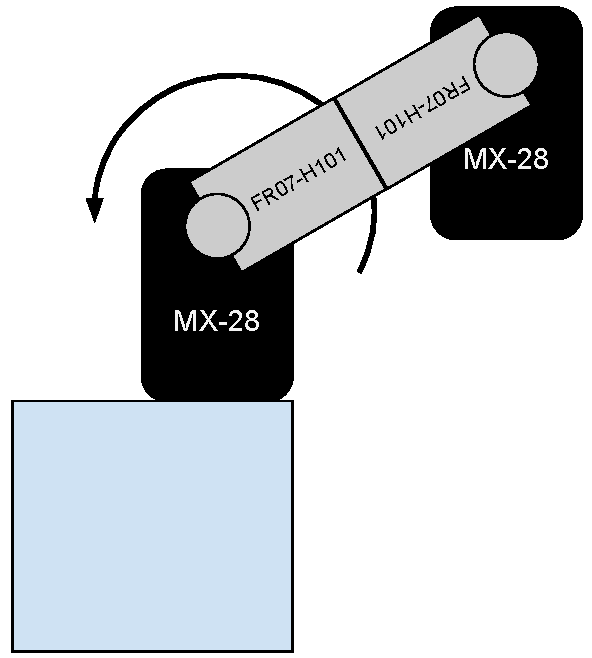
\includegraphics[width = 0.3\textwidth]{figures/exp2}
    \caption[Experimental setup dynamics testing]{Experimental setup for dynamics testing. One servo lifts the other one. The goal is the measure the time it takes to swing the arm from $0\degree$ to $180\degree$.}
    \label{fig:exp2}
\end{figure}


\section{Conclusion}